\section{Molek�le}
LCAO-Approximation: Linear Combination of Atomic Orbitals.
\subsection{$H_2^+$ Molek�l (ein Elektron, zwei Protonen)}
\begin{tabular}{p{4cm} p{15cm}}
Hamilton-Operator	& $\hat H = -\frac{\hbar^2}{2m} \nabla^2 + \frac{e^2}{4\pi\epsilon_0} \left(-\frac{1}{r_1}- \frac{1}{r_2} + \frac{1}{r} \right)$ $r$: Abstand Proton-Proton, $r_{1,2}$: Abstand Elektron-Proton\\
LCAO-Approximation	& Spalte $H_2^+$ gedanklich auf in $H$ und $H^+$, dann gibt es eine Wellenfunktion $\Psi_1$, bei der das $H$ links ist und eine Wellenfunktion $\Psi_2$, bei der das $H$ rechts ist. Diese aufgespaltenen Zust�nde bringt man durch Linearkombination wieder zusammen.\\
Gesamtwellenfkt.	& \begin{tabular}[t]{l}
                	   $\Psi_{gerade} = \Psi_1 + \Psi_2$\\
			   $\Psi_{ungerade} = \Psi_1 - \Psi_2$\\
			   $\Rightarrow$ Durch die �berlappung (LCAO) entstehen zwei Molek�lorbitale
                	  \end{tabular}\\
Mittlere Energie des Elektrons	& $E = \frac{\int \Psi^{\asterisk} H \Psi dV}{\int \Psi^{\asterisk} \Psi dV} = E_a + \frac{e^2}{4\pi\epsilon_0 r} - \frac{A\pm B}{1\pm S}\quad +: \Psi_{gerade}, -:\Psi_{ungerade}$\\
�berlappintegral (Proton-Proton)	& $S = S(r) = \int \Psi(r_1) \Psi_2(r_1)dV_1\quad \lim_{r\to 0} S = S_{max}$\\
Anziehungsenergie (Elektron-Proton 2)	& $A = A(r) = \frac{e^2}{4\pi\epsilon_0}\int \frac{\Psi_1^2(r_1)}{r_2}dV_1$\\
�berlappungsterm (Elektron-Proton 1)	& $B = B(r) = \frac{e^2}{4\pi\epsilon_0} \int \frac{\Psi_1(r_1)\Psi_2(r_2)}{r_1}dV_1$\\
Kovalente Bindung	& $\Psi_1 + \Psi_2$ ist bindend und macht die kovalente Bindung. $\Psi_1 - \Psi_2$ ist dagegen nichtbindend.\\
			& 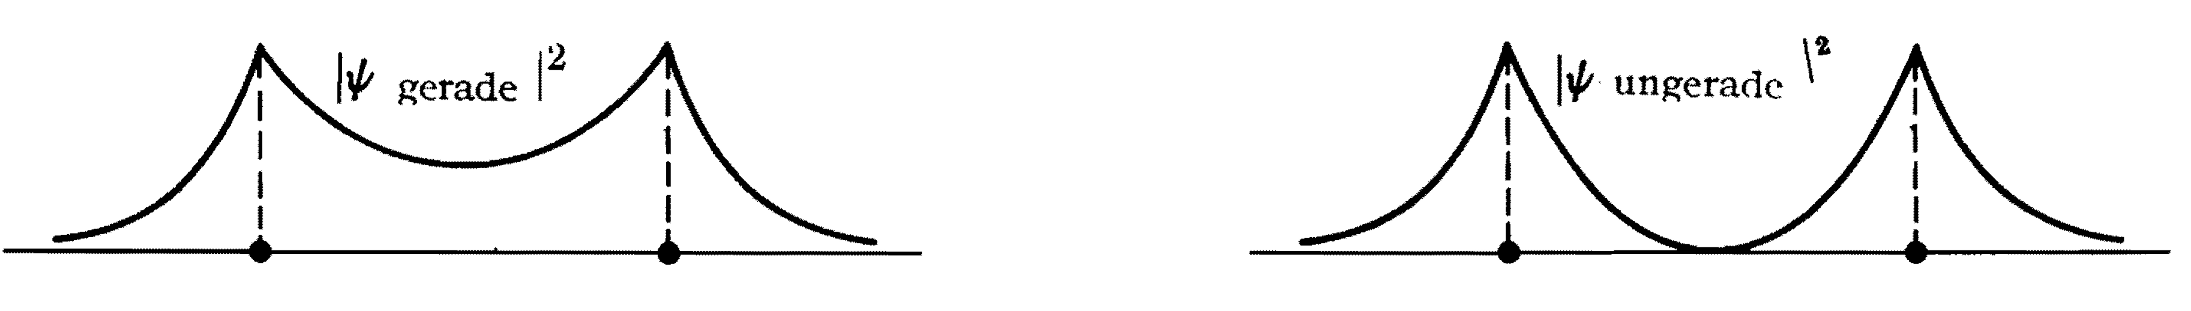
\includegraphics[width = 14cm]{ph_kovalentebdg.png}
\end{tabular}
\subsection{$H_2$ Molek�l (zwei Elektronen, zwei Protonen)}
Das Ganze funktioniert im Prinzip analog, nur dass man jetzt Atomorbitale linear kombiniert.\\
\begin{tabular}{p{4cm} p{15cm}}
Pauli-Prinzip	& Da wir mehr als ein Elektron haben, muss die Gesamtwellenfkt. antisymmetrisch sein.\\
Drehimpuls	& Drehimpuls $L$ eines $e^-$ nicht konstant, da kein Zentralfeld (lineares Molek�l)\\
		& $L_z = m_l\hbar$ konstant, da Kraft auf Elektronen immer durch Protonenachse\\
Drehimpulszust�nde im Molek�l	& \begin{tabular}[t]{lcccc}
                             	   $m_l$		& 0        & $\pm$ 1 & $\pm$ 2  & $\pm$ 3\\
				   Symbol		& $\sigma$ & $\pi$   & $\delta$ & $\Phi$\\
				   $\# e^-$		& 2	   & 4	 & 4	  & 4\\
				   \multicolumn{5}{l}{$\# e^-$ wegen Spin up, down}
                             	  \end{tabular}\\
LCAO		& Nun werden Atomorbitale analog zu oben linear kombiniert. Das resultierende MO h�ngt von den $m_l$ der Elektronen in den Atomorbitalen ab.\\
Beispiele	& 2 ns Atomorbitale ergeben ein $\sigma$ Molek�lorbital, weil $m_l = 0$ f�r ns Atomorbitale\\
		& 2 np Atomorbitale ergeben entweder ein $\sigma$ MO ($np_z$) oder ein $\pi$ MO ($np_x, np_y$), da $m_l$ f�r die p-AO -1,0,1 ist.\\
gerade, ungerade	& Subscript g: gerade Wellenfunktion (= MO), Subscript u: ungerade, Bsp: $\sigma_u$\\
bindend, nichtbindend	& Superscript $\ast$: nichtbindende Wellenfunktion (= MO), Bsp: $\sigma_u^{\ast}$\\
Elektronenkonfiguration	& 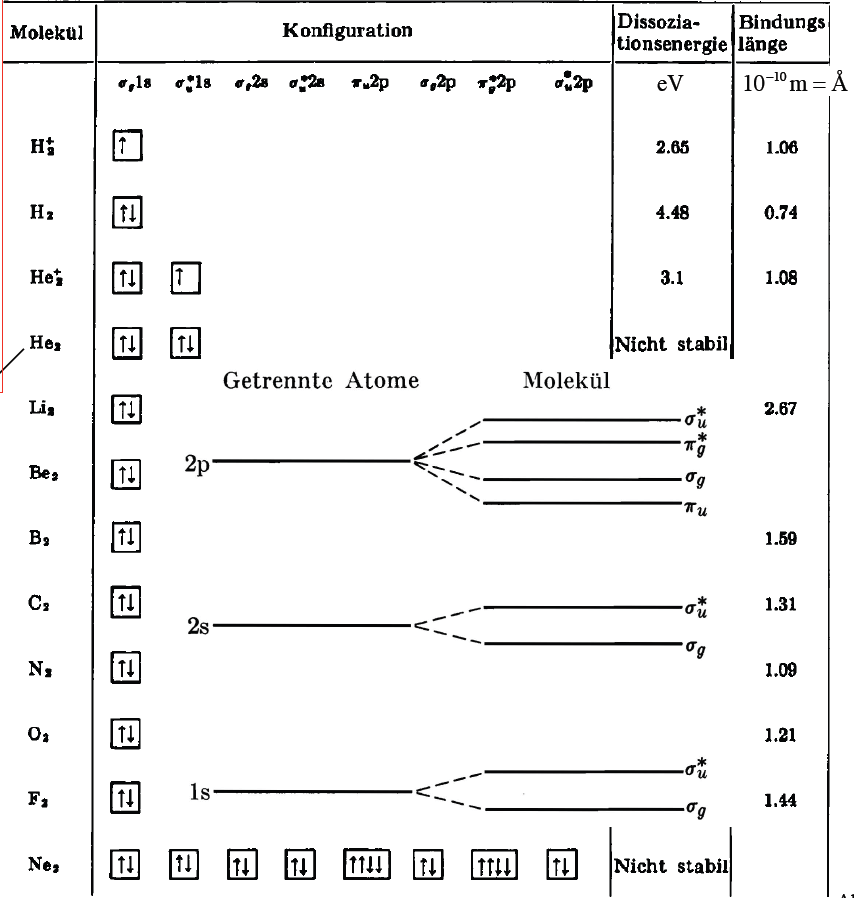
\includegraphics[width = 15cm]{ph_elektronenkonfi.png}
\end{tabular}
\subsection{Hybrid-Wellenfunktionen}
\begin{tabular}{p{4cm} p{15cm}}
 sp	& \\
$sp^2$	& planar-trigonal\\
$sp^3$	& tetraedrisch $(CH_4)$\\
	& \begin{tabular}[t]{ll}
	  $\Psi_1 = \tfrac{1}{2} (s + p_x + p_y + p_z)$	& $\Psi_2 = \tfrac{1}{2} (s + p_x - p_y - p_z)$\\
	  $\Psi_3 = \tfrac{1}{2} (s - p_x + p_y - p_z)$	& $\Psi_4 = \tfrac{1}{2} (s - p_x - p_y + p_z)$
	  \end{tabular}
\end{tabular}
\subsection{Molekulare Rotation}
\begin{tabular}{p{4cm}p{15cm}}
Rotationsenergie eines 2-atomigen Molek�ls	& $E_r = \frac{L^2}{2I} = \frac{\hbar^2}{2I} l(l+1)\quad I =$ Tr�gheitsmoment\\
Auswahlregel (elektr. Dipolstrahlung)		& $\Delta l = \pm 1 \Rightarrow \Delta E_{l,l-1} = 2lE_1\quad E_1 = \frac{\hbar^2}{2I}$\\
\end{tabular}
\subsection{Molekulare Vibration}
Modelliert durch harmonischen Oszillator.\\
\begin{tabular}{p{4cm}p{15cm}}
Vibrationsenergie	& $E_n = \left(n+\frac{1}{2}\right) \hbar\omega$\\
\multicolumn{2}{l}{Pro Vibrationsenergieniveau gibt es also mehrere ($n-1$ viele) Rotationsenergieniveaus.}
\end{tabular}